\documentclass{beamer}
\usepackage{booktabs}
\usepackage{graphicx}
\usetheme{default}
\setbeamertemplate{navigation symbols}{}
\setbeamertemplate{footline}{\hfill\insertframenumber/\inserttotalframenumber\hspace{1.5em}}

\title{Robust Constraint Learning for Chemotherapy Regimen Design}
\date{}

\begin{document}

\begin{frame}
  \titlepage
\end{frame}

\begin{frame}{Problem setup}
- Constraint learning: embed a trained model $\hat f(x)\le b$ inside an optimization.
- Noisy training labels $\Rightarrow$ the ``optimal'' decision can violate the \emph{true} constraint.
- Goal: make the embedded-constraint decision robust to \textbf{label (y) noise}.
- Case study: OptiCL gastric-cancer chemotherapy (Maragno et al., Table~6) --- maximize
  overall survival (OS) s.t.\ five grade 3--4 toxicity constraints $\le$ the 60th percentile.
\end{frame}

\begin{frame}{Method: Robust Cutting Planes (CP)}
- \textbf{Robustify the \emph{decision}}, not the model: keep a nominal fit, hedge at the
  prescription via localized-bootstrap separation of worst-case models around $x^\ast$.
- Trilevel formulation solved by iteratively adding cuts for the worst sampled scenario;
  self-regulates via a coverage cap $\alpha$ (no OS-objective robustification, one global master).
- Contrast --- the baselines instead \textbf{robustify the \emph{model}}:
  \begin{itemize}
  \item \emph{Nominal}: point estimate, no robustness.
  \item \emph{Robust Reg.}: label-robust training counterpart (Bertsimas et al.\ 2019), embedded nominally.
  \item \emph{Wrapper}: joint chance constraint over a bootstrap ensemble.
  \end{itemize}
\end{frame}

\begin{frame}{Evaluation: measuring label-noise robustness}
- GT ensemble = fixed oracle: 6 models/outcome (CV-selected), averaged, fit once on the full
  clean cohort. Feasibility: mean GT prediction $\le$ threshold.
- A single training draw cannot reveal robustness (feasibility near-saturated). So we probe the
  \emph{distribution} over draws.
- \textbf{Label-noise probe}: repeat over $R$ training subsamples (m-out-of-n, without
  replacement); refit only the constraint/robust models; score against the fixed oracle.
- Roles separated: oracle fixed; each method keeps its own ambiguity set; outer subsampling is the
  probe. Report mean, SD, and \textbf{worst-case} feasibility across draws.
\end{frame}

\begin{frame}{Headline: CP dominates at the reference threshold}
  \centering
  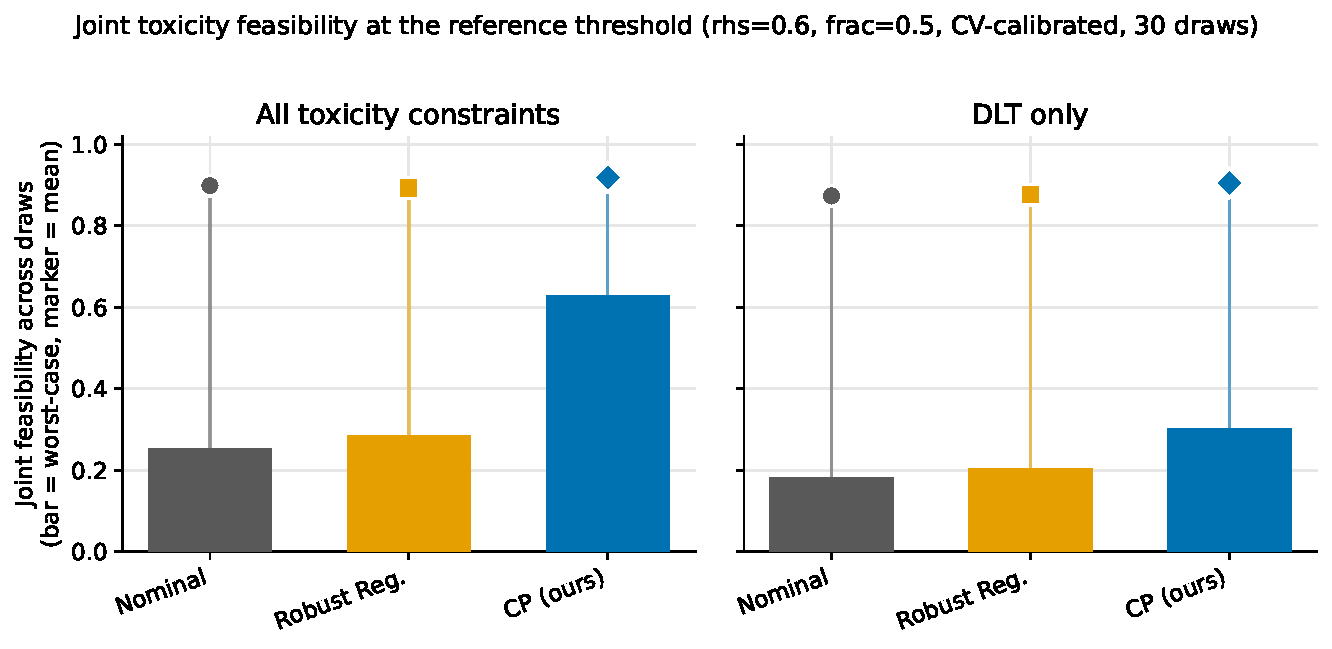
\includegraphics[width=\linewidth]{../results/figures/fig_headline.pdf}

  \raggedright\small
  At rhs$=0.6$, frac$=0.5$ (all-constraints): CP worst-case \textbf{0.64} vs nominal 0.18,
  SD \textbf{0.07} vs 0.17, mean \textbf{0.94} vs 0.90 --- best on every feasibility axis.
\end{frame}

\begin{frame}{The robustness--survival trade-off}
  \centering
  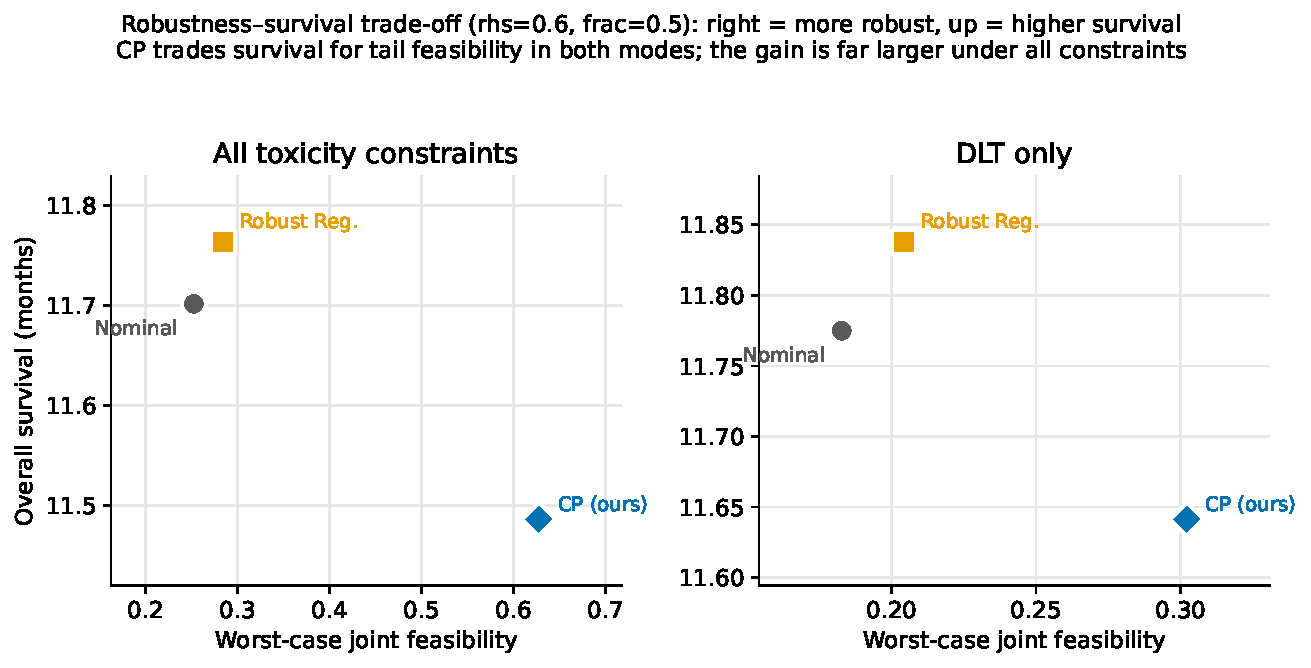
\includegraphics[width=\linewidth]{../results/figures/fig_tradeoff.pdf}

  \raggedright\small
  CP buys a large worst-case-feasibility gain for a small OS cost ($\sim$0.1--0.4 mo).
  Robust~Reg.\ $\approx$ nominal (model-robustness does not protect the decision).
\end{frame}

\begin{frame}{Frontier 1: vs constraint tightness}
  \centering
  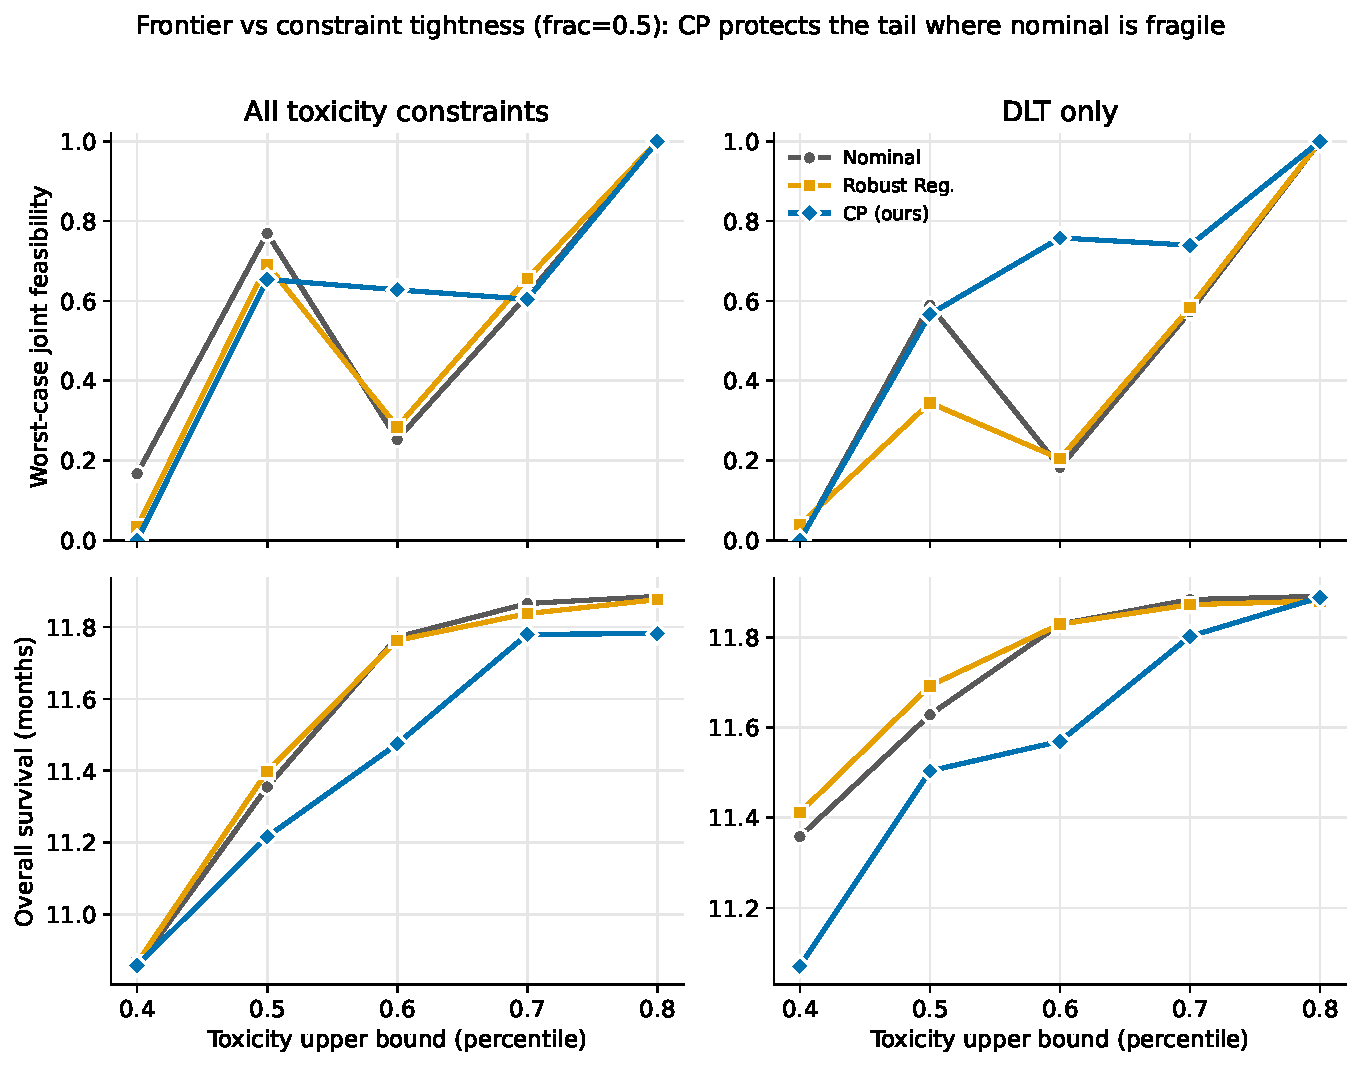
\includegraphics[width=0.92\linewidth]{../results/figures/fig_rhs_frontier.pdf}

  \raggedright\small
  CP's edge appears in the fragile zone (rhs $0.6$--$0.7$) where the loose constraint lets nominal
  push to the boundary; it ties when binding-tight ($0.4$--$0.5$) or vacuous ($0.8$).
\end{frame}

\begin{frame}{Frontier 2: vs data scarcity}
  \centering
  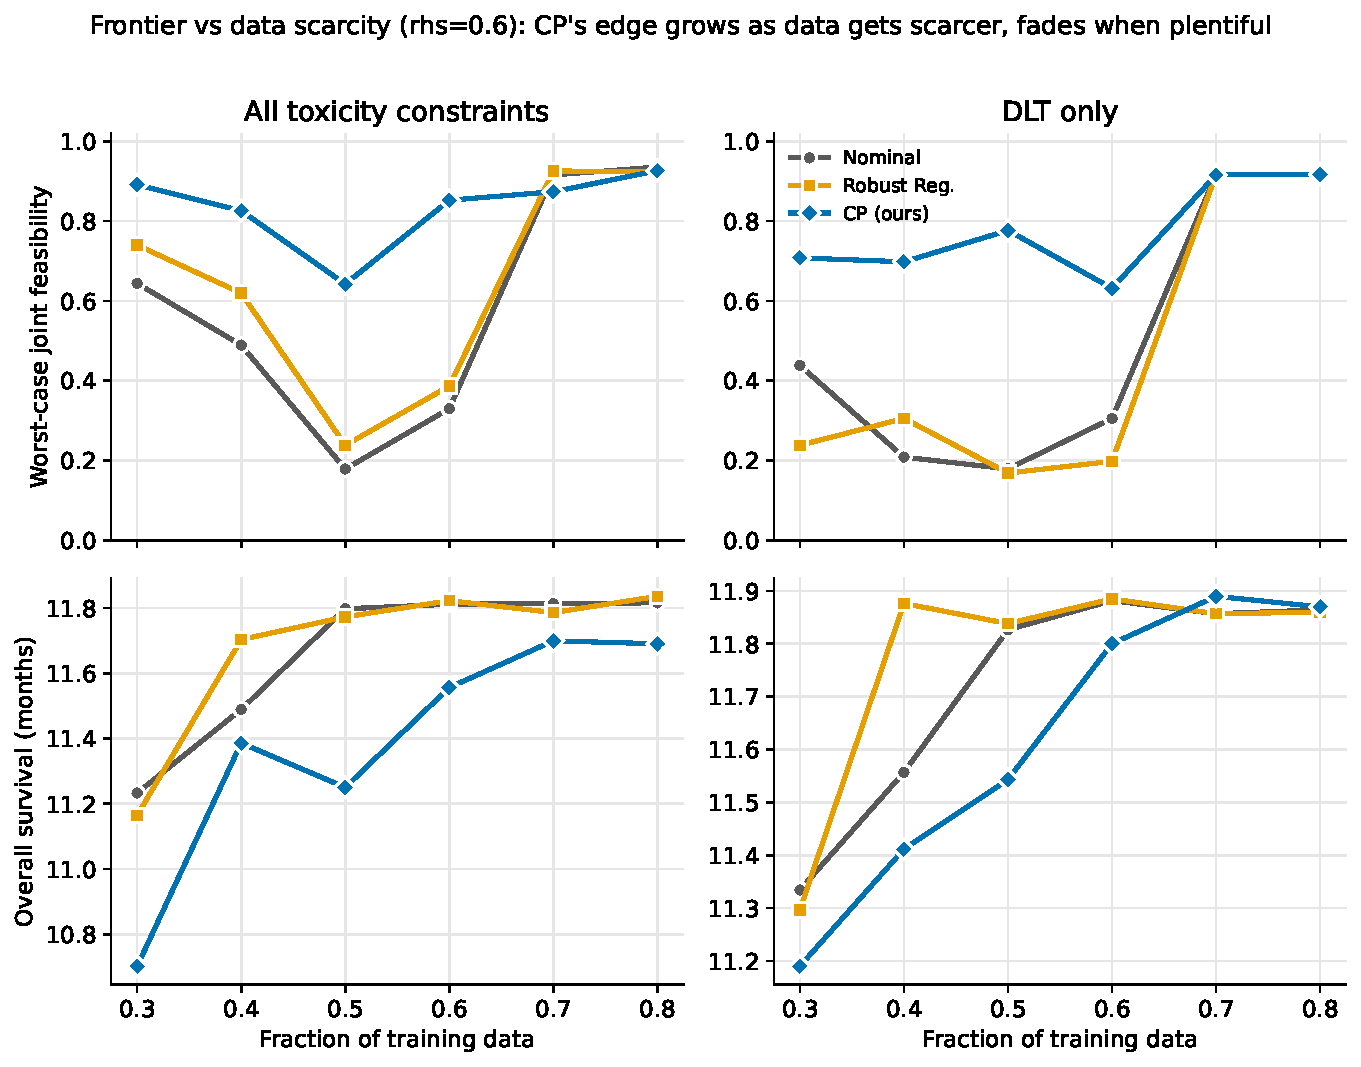
\includegraphics[width=0.92\linewidth]{../results/figures/fig_frac_frontier.pdf}

  \raggedright\small
  CP's worst-case edge grows as data gets scarcer ($0.3$--$0.6$) and fades when plentiful
  ($0.7$--$0.8$, where nominal is already stable). OS cost shrinks in parallel.
\end{frame}

\begin{frame}{Takeaways \& next steps}
- \textbf{CP delivers tail-robustness exactly where it should}: uncertain estimates (scarce data)
  and decisions near the boundary (loose constraint); it costs little when robustness isn't needed.
- Robustifying the \emph{decision} (CP) beats robustifying the \emph{model} (Robust Reg.) for
  downstream feasibility; wrapper is competitive on worst-case but costs more OS.
- Next: synthetic problem (CP is the only truly feasible method as noise grows); other ambiguity
  sets (conformal, Wasserstein-DRO); tractable robust counterparts for linear/SVM.
\end{frame}

\end{document}
